Nel paragrafo precedente abbiamo descritto due modelli di telescopi: il rifrattore di Galilei, che sfrutta il potere rifrattivo del vetro per creare un'immagine nel fuoco, e il riflettore di Newton, che sfruttano il fatto che la radiazione incidente su una superficie viene riflessa in un unico punto detto fuoco.

Vediamo i problemi che presentano questi modelli:

\subsubsection{Problemi dei rifattori}

\begin{itemize}
\item Le lenti usate hanno un fuoco che dipende dalla lunghezza d'onda e questo costituisce il fenomeno della cosiddetta \textbf{aberrazione cromatica}:

\vspace{-0.3cm}

\begin{minipage}{0.45\textwidth}
    \begin{figure}[H]
        \centering
        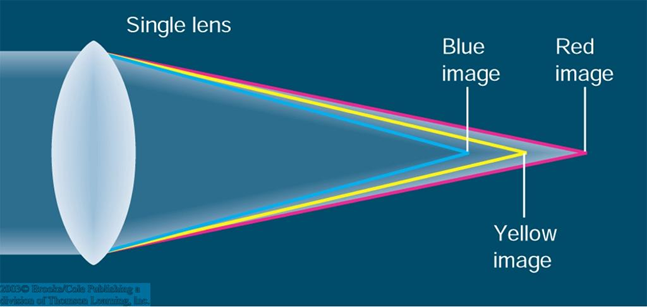
\includegraphics[width=6cm]{immagini/aberrazione_cromatica.png}
    \end{figure}
\end{minipage}
\begin{minipage}{0.5\textwidth}
    \begin{figure}[H]
        \centering
        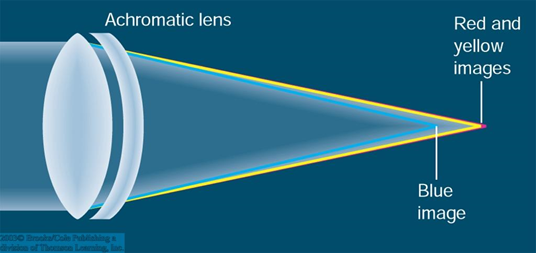
\includegraphics[width=6cm]{immagini/lenti_acromatiche.png}
    \end{figure}
\end{minipage}

\vspace{0.2cm}

supponiamo, allora, di voler osservare una stella di luce policromatica: sull'asse del telescopio si formeranno tante immagini monocromatiche della sorgente quanti sono i colori della sorgente stessa, in punti diversi dell'asse ottico (i diversi fuochi, ognuno corrispondente ad una lunghezza d'onda), come si vede nella figura a sinistra. Non avremo, dunque, un'unica immagine complessiva.

Si risolse in parte il problema usando \textit{lenti acromatiche} (come quella in figura a destra), cioè lenti secondarie che hanno l'obiettivo di spostare il fuoco di alcune lunghezze d'onda di una data quantità, in modo da far coincidere tutti i fuochi della lente del telescopio in un unico punto e formare un unica immagine.

\item Maggiore è l'area della lente (ciò che idealmente vorremmo sempre, perché un telescopio più grande equivale a misure migliori), maggiore è il suo spessore. Ciò comporta un aumento in peso. Dunque, aumenta il rischio che vi siano fenomeni di \textbf{assorbimento} della radiazione durante il suo passaggio attraverso la lente.

\item I rifrattori erano soliti avere delle focali molto lunghe per evitare il problema della distorsione dell'immagine in una direzione; infatti, imperfezioni nella lavorazione della lente facevano sì che non tutti i raggi rifratti si concentrassero esattamente in corrispondenza del fuoco, facendo apparire l'immagine un po' allungata. Tuttavia, in questo modo il telescopio risultava eccessivamente grande e difficile da maneggiare.
\end{itemize}

\subsubsection{I problemi dei riflettori}

I primi riflettori furono delle sfere perché facili da realizzare; purtroppo però una sfera riflettente è sempre soggetta al problema dell'\textbf{aberrazione sferica}.

\begin{minipage}{0.345\textwidth}
    \begin{figure}[H]
        \centering
        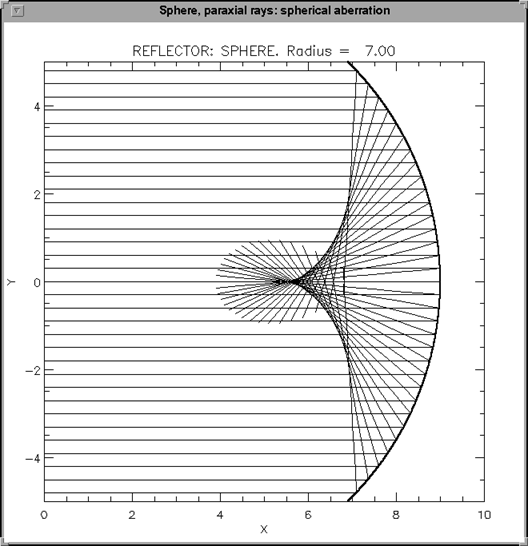
\includegraphics[width=5cm]{immagini/aberrazione_sferica.png}
    \end{figure}
\end{minipage}
\begin{minipage}{0.65\textwidth}
    \vspace{0.5cm}Questo consiste nell'inesistenza di un vero e proprio fuoco per questo tipo di telescopi, a causa del fatto che la posizione in cui viene riflesso un certo raggio (incidente parallelamente all'asse ottico) dipende dalla distanza del punto di incidenza del raggio dal vertice dello specchio. I vari raggi verranno riflessi in punti diversi dell'asse. Di conseguenza, non esiste per essi un punto in cui la sorgente diventi esattamente puntiforme; piuttosto, l'immagine è sempre vista come un punto con intorno un certo anello circolare concentrico al punto, più o meno largo.
\end{minipage}

\vspace{0.2cm}Il meglio che si possa fare è di individuare e osservare la sorgente luminosa nella posizione in cui l'anello presenta il diametro minore (\textit{cerchio di minima confusione}).

La forma perfetta che permette, al contrario della sfera, di raccogliere in un unico punto (fuoco) i raggi provenienti dall'infinito è il paraboloide.

\begin{figure}[H]
    \centering
    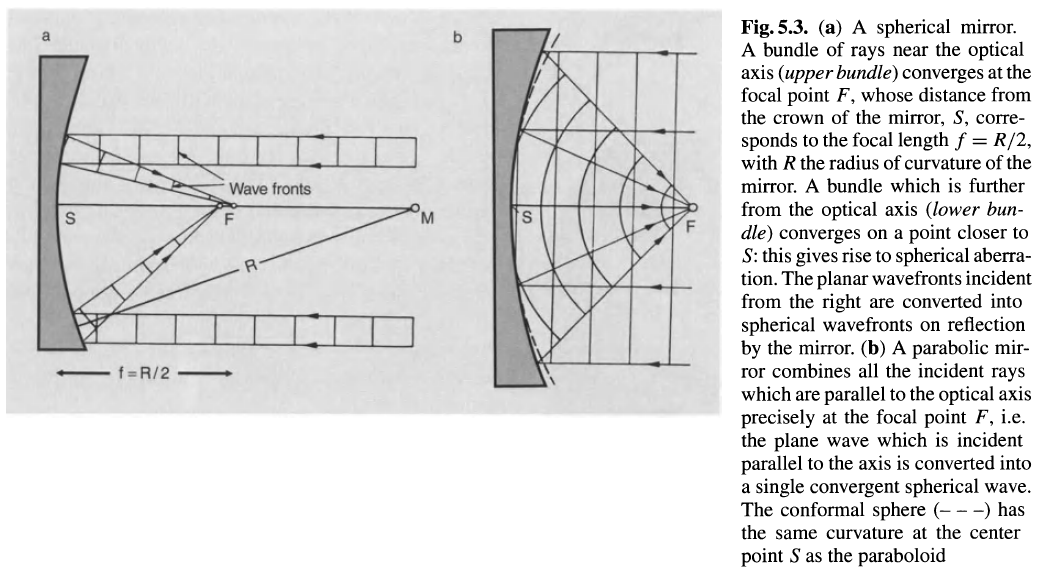
\includegraphics[width=14cm]{immagini/sfera_vs_paraboloide.png}
\end{figure}

Anche questo telescopio presenta un problema: nel caso in cui i raggi non incidano parallelamente all'asse ottico, il fuoco sarà un oggetto esteso e non più puntiforme. Allora, l'immagine di una stella non collocata sull'asse del telescopio sarà allungata in una direzione. Si parla di \textbf{coma}.

\begin{minipage}{0.5\textwidth}
    \begin{figure}[H]
        \centering
        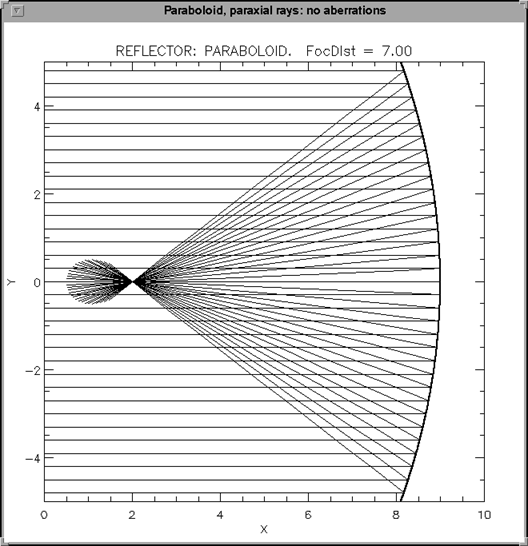
\includegraphics[width=5cm]{immagini/specchio_parabolico.png}
    \end{figure}
\end{minipage}
\begin{minipage}{0.5\textwidth}
    \begin{figure}[H]
        \centering
        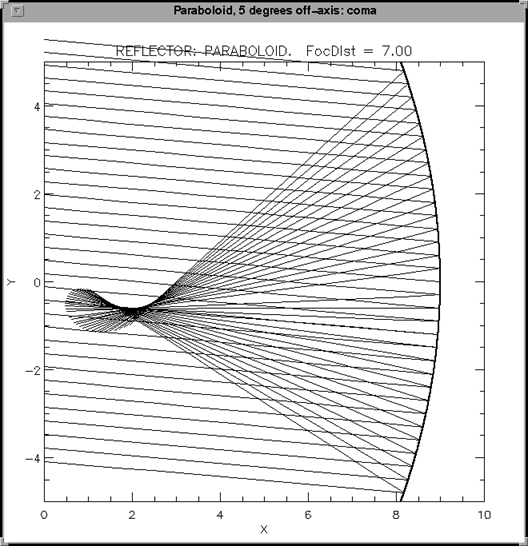
\includegraphics[width=5cm]{immagini/coma_1.png}
    \end{figure}
\end{minipage}

\vspace{0.4cm}Un altro difetto è \textbf{l'astigmatismo}. I telescopi, infatti, idealmente prevederebbero una perfetta simmetria assiale dell'occhio umano (l'occhio vede una certa figura alla stessa maniera comunque essa venga ruotata), cosa che in realtà non succede mai. Le immagini risultano allora allungate in una direzione. Questo problema si risolve con delle lenti sferiche, che permettono all'imagine di allungarsi o schiacciarsi in una direzione ben precisa.

Nonostante queste complicanze, nel tempo i riflettori furono preferiti ai rifrattori.

